\documentclass{article}
\usepackage[table]{xcolor}
\usepackage{array}
\usepackage{float}
\usepackage{graphicx}
\usepackage{tikz}
\usepackage{tcolorbox}
\usepackage{amsmath}
\usepackage{enumitem}
\usetikzlibrary{trees, arrows.meta}
\usepackage{listings}
\usepackage{xcolor}
\usepackage[utf8]{inputenc}   % Suporte para codificação UTF-8
% Definir um verde mais suave
\definecolor{mygreen}{rgb}{0.1, 0.6, 0.1}
\lstset{
    language=Python,
    basicstyle=\ttfamily\footnotesize,
    keywordstyle=\color{blue},
    commentstyle=\color{mygreen},
    stringstyle=\color{red},
    numbers=left,
    numberstyle=\tiny\color{gray},
    stepnumber=1,
    numbersep=10pt,
    showstringspaces=false,
    frame=single,
    tabsize=4,
    breaklines=true,
    breakatwhitespace=false,
    escapeinside={\%*}{*)},
    literate={á}{{\'a}}1 {é}{{\'e}}1 {í}{{\'i}}1 {ó}{{\'o}}1 {ú}{{\'u}}1
             {Á}{{\'A}}1 {É}{{\'E}}1 {Í}{{\'I}}1 {Ó}{{\'O}}1 {Ú}{{\'U}}1
             {à}{{\`a}}1 {è}{{\`e}}1 {ì}{{\`i}}1 {ò}{{\`o}}1 {ù}{{\`u}}1
             {À}{{\`A}}1 {È}{{\`E}}1 {Ì}{{\`I}}1 {Ò}{{\`O}}1 {Ù}{{\`U}}1
             {â}{{\^a}}1 {ê}{{\^e}}1 {î}{{\^i}}1 {ô}{{\^o}}1 {û}{{\^u}}1
             {Â}{{\^A}}1 {Ê}{{\^E}}1 {Î}{{\^I}}1 {Ô}{{\^O}}1 {Û}{{\^U}}1
             {ä}{{\"a}}1 {ë}{{\"e}}1 {ï}{{\"i}}1 {ö}{{\"o}}1 {ü}{{\"u}}1
             {Ä}{{\"A}}1 {Ë}{{\"E}}1 {Ï}{{\"I}}1 {Ö}{{\"O}}1 {Ü}{{\"U}}1
             {ã}{{\~a}}1 {õ}{{\~o}}1 {Ã}{{\~A}}1 {Õ}{{\~O}}1
}

\renewcommand\thesubsection{\arabic{subsection}} % Hace que subsección use solo números (1, 2, 3, etc.)
\setcounter{secnumdepth}{2} % Asegura que las subsecciones se numerarán

\title{AULA 08: Exercício teórico Métodos de Pesquisa e Árvores AVL}
\author{Aluno: Gian Franco Joel Condori Luna}
\date{\today}

\begin{document}

\maketitle

\section*{Exercices}
\setcounter{section}{1}
\subsection {(0,4) Insira as seguintes chaves: {924, 220, 911, 244, 898, 258, 362, 363, 360, 350}.}

\begin{enumerate}[label=\alph*)]
  \item em uma árvore binária comum.
  \item depois em uma árvore AVL mostrando as rotações passo-a-passo.
  \item remova o nó 362 em ambas as árvores.
\end{enumerate}

\subsubsection{Solução:}

\subsubsection{a) em uma árvore binária comum.}

\begin{enumerate}
  \item Inserindo 924:
  \begin{center}
    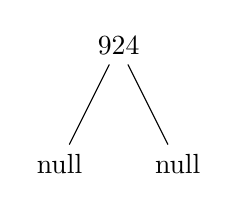
\begin{tikzpicture}
        \node {924}
          child {node {null}}
          child {node {null}};
    \end{tikzpicture}
  \end{center}

  \item Inserindo 220:
  \begin{center}
    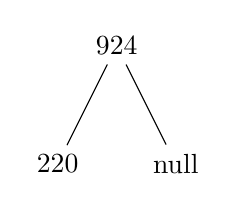
\begin{tikzpicture}
        \node {924}
            child {node {220}}
            child {node {null}};
    \end{tikzpicture}
    \end{center}
    
  \item Inserindo 911:
  \begin{center}
    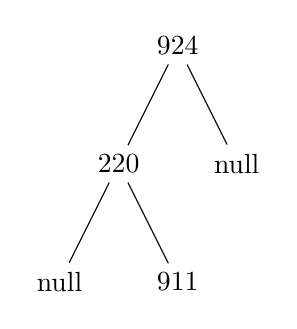
\begin{tikzpicture}
        \node {924}
            child {
              node {220}
              child {node {null}}
              child {node {911}}
            }
            child {
              node {null}
            };
    \end{tikzpicture}
  \end{center}
    
  \item Inserindo 244:
  \begin{center}
    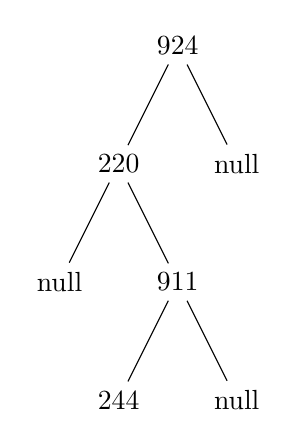
\begin{tikzpicture}
        \node {924}
            child {
              node {220}
              child {node {null}}
              child {node {911}
                child {node {244}}
                child {node {null}}
              }
            }
            child {
              node {null}
            };
    \end{tikzpicture}
  \end{center}
    
  \item Inserindo 898:
  \begin{center}
    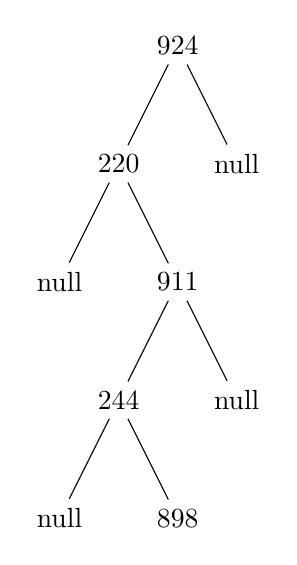
\begin{tikzpicture}
        \node {924}
            child {
              node {220}
              child {node {null}}
              child {node {911}
                child {node {244}
                  child {node {null}}
                  child {node {898}}
                }
                child {node {null}}
              }
            }
            child {
              node {null}
            };
    \end{tikzpicture}
  \end{center}
    
  \item Inserindo 258:
  \begin{center}
    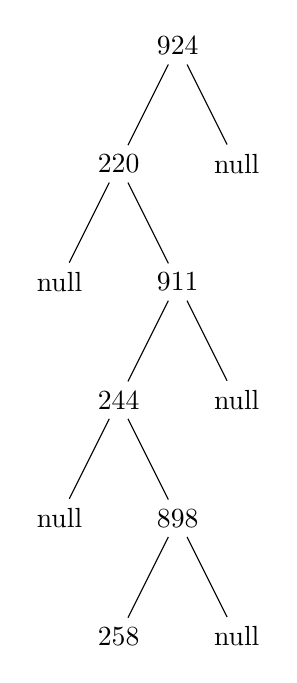
\begin{tikzpicture}
        \node {924}
            child {
              node {220}
              child {node {null}}
              child {node {911}
                child {node {244}
                  child {node {null}}
                  child {node {898}
                    child {node {258}}
                    child {node {null}}
                  }
                }
                child {node {null}}
              }
            }
            child {
              node {null}
            };
    \end{tikzpicture}
  \end{center}
    
  \item Inserindo 362:
  \begin{center}
    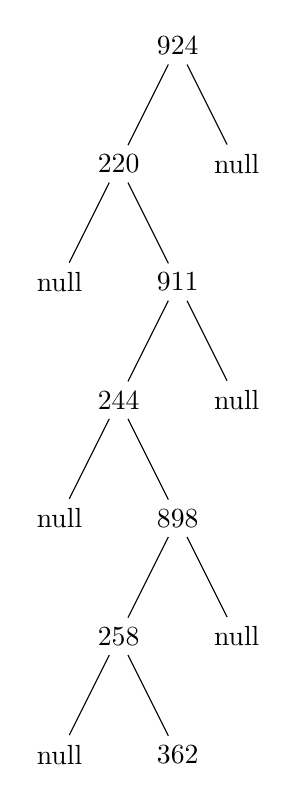
\begin{tikzpicture}
        \node {924}
            child {
              node {220}
              child {node {null}}
              child {node {911}
                child {node {244}
                  child {node {null}}
                  child {node {898}
                    child {node {258}
                      child {node {null}}
                      child {node {362}}
                    }
                    child {node {null}}
                  }
                }
                child {node {null}}
              }
            }
            child {
              node {null}
            };
    \end{tikzpicture}
  \end{center}

  \item Inserindo 363:
  \begin{center}
    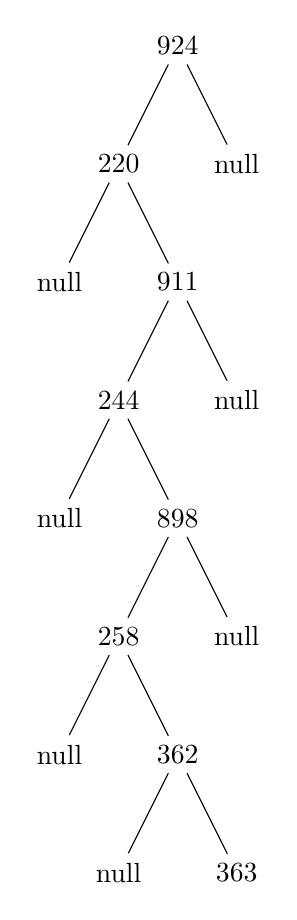
\begin{tikzpicture}
        \node {924}
            child {
              node {220}
              child {node {null}}
              child {node {911}
                child {node {244}
                  child {node {null}}
                  child {node {898}
                    child {node {258}
                      child {node {null}}
                      child {node {362}
                        child {node {null}}
                        child {node {363}}
                      }
                    }
                    child {node {null}}
                  }
                }
                child {node {null}}
              }
            }
            child {
              node {null}
            };
    \end{tikzpicture}
  \end{center}

  \item Inserindo 360:
  \begin{center}
    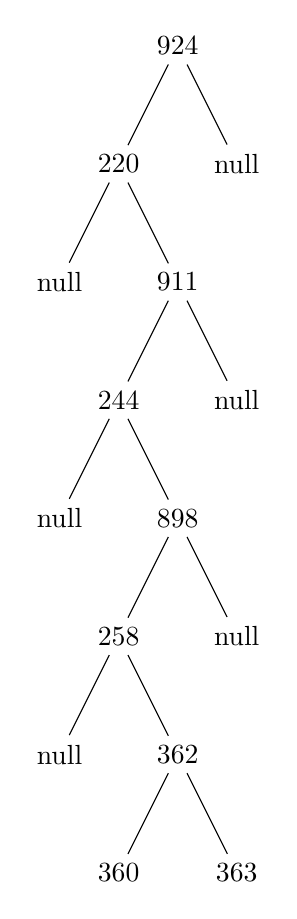
\begin{tikzpicture}
        \node {924}
            child {
              node {220}
              child {node {null}}
              child {node {911}
                child {node {244}
                  child {node {null}}
                  child {node {898}
                    child {node {258}
                      child {node {null}}
                      child {node {362}
                        child {node {360}}
                        child {node {363}}
                      }
                    }
                    child {node {null}}
                  }
                }
                child {node {null}}
              }
            }
            child {
              node {null}
            };
    \end{tikzpicture}
  \end{center}

  \item Inserindo 350:
  \begin{center}
    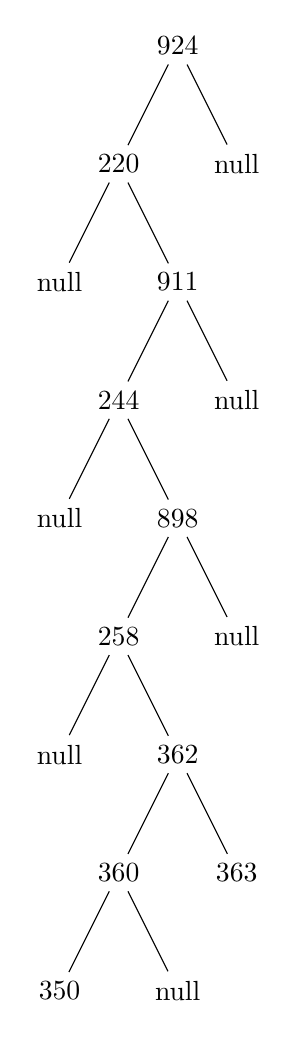
\begin{tikzpicture}
        \node {924}
            child {
              node {220}
              child {node {null}}
              child {node {911}
                child {node {244}
                  child {node {null}}
                  child {node {898}
                    child {node {258}
                      child {node {null}}
                      child {node {362}
                        child {node {360}
                          child {node {350}}
                          child {node {null}}
                        }
                        child {node {363}}
                      }
                    }
                    child {node {null}}
                  }
                }
                child {node {null}}
              }
            }
            child {
              node {null}
            };
    \end{tikzpicture}
  \end{center}

\end{enumerate}

\subsubsection{b) depois em uma árvore AVL mostrando as rotações passo-a-passo.}

\begin{enumerate}
  \item Inserindo 924:
  \begin{center}
    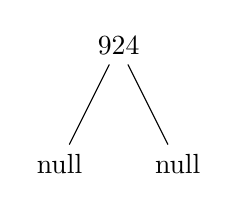
\begin{tikzpicture}
        \node {924}
          child {node {null}}
          child {node {null}};
    \end{tikzpicture}
  \end{center}

  \item Inserindo 220:
  \begin{center}
    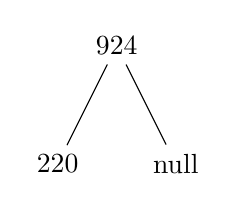
\begin{tikzpicture}
        \node {924}
            child {node {220}}
            child {node {null}};
    \end{tikzpicture}
    \end{center}
    
  \item Inserindo 911:
  \begin{center}
    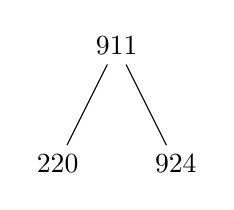
\begin{tikzpicture}
        \node {911}
            child {
              node {220}
            }
            child {
              node {924}
            };
    \end{tikzpicture}
  \end{center}

  \item Inserindo 244:
  \begin{center}
    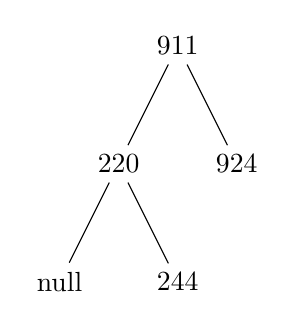
\begin{tikzpicture}
        \node {911}
            child {
              node {220}
              child {node {null}}
              child {node {244}}
            }
            child {
              node {924}
            };
    \end{tikzpicture}

  \end{center}

  \item Inserindo 898:
  \begin{center}
    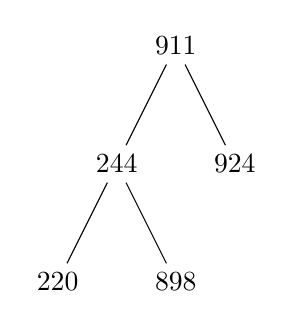
\begin{tikzpicture}
        \node {911}
            child {
              node {244}
              child {node {220}}
              child {node {898}}
            }
            child {
              node {924}
            };
    \end{tikzpicture}
  \end{center}

  \item Inserindo 258:
  \begin{center}
    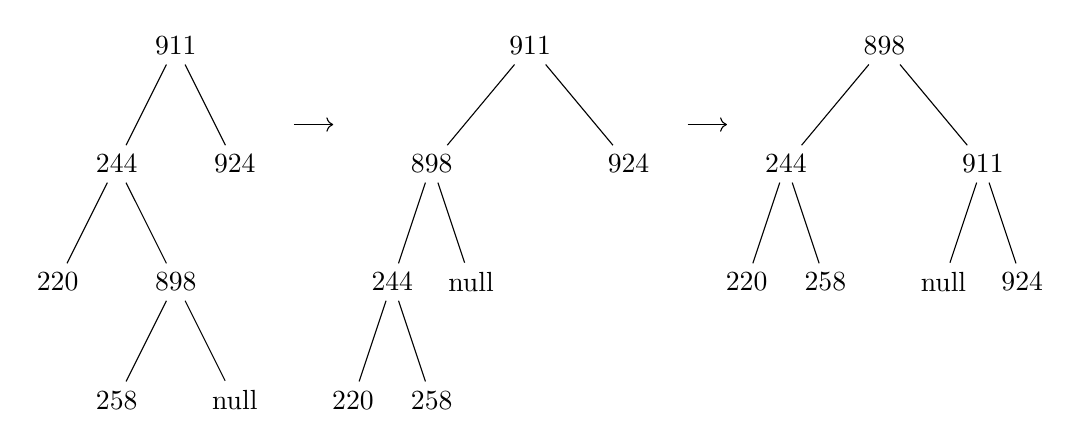
\begin{tikzpicture}
        % Primeiro arvore
        \node {911}
            child {
              node {244}
              child {node {220}}
              child {node {898}
                child {node {258}}
                child {node {null}}
              }
            }
            child {
              node {924}
            };

        \draw[->] (1.5,-1) -- (2,-1);

        % Segundo arvore
        \node[shift={(4.5,0)}] {911}
            child[sibling distance=2.5cm] {
              node {898}
              child[sibling distance=1cm] {node {244}
                child[sibling distance=1cm] {node {220}}
                child[sibling distance=1cm] {node {258}}
              }
              child[sibling distance=1cm] {node {null}}
            }
            child[sibling distance=2.5cm] {
              node {924}
            };
        
        \draw[->] (6.5,-1) -- (7,-1);

        % Terceiro arvore
        \node[shift={(9,0)}] {898}
            child[sibling distance=2.5cm] {
              node {244}
              child[sibling distance=1cm] {node {220}}
              child[sibling distance=1cm] {node {258}}
            }
            child[sibling distance=2.5cm] {
              node {911}
              child[sibling distance=1cm] {node {null}}
              child[sibling distance=1cm] {node {924}}
            };
    \end{tikzpicture}
  \end{center}

  \item Inserindo 362:
  \begin{center}
    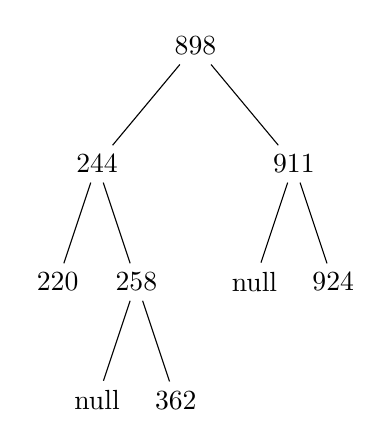
\begin{tikzpicture}
        \node {898}
            child[sibling distance=2.5cm] {
              node {244}
              child[sibling distance=1cm] {node {220}}
              child[sibling distance=1cm] {node {258}
                child[sibling distance=1cm] {node {null}}
                child[sibling distance=1cm] {node {362}}
              }
            }
            child[sibling distance=2.5cm] {
              node {911}
              child[sibling distance=1cm] {node {null}}
              child[sibling distance=1cm] {node {924}}
            };
    \end{tikzpicture}
  \end{center}

  \item Inserindo 363:
  \begin{center}
    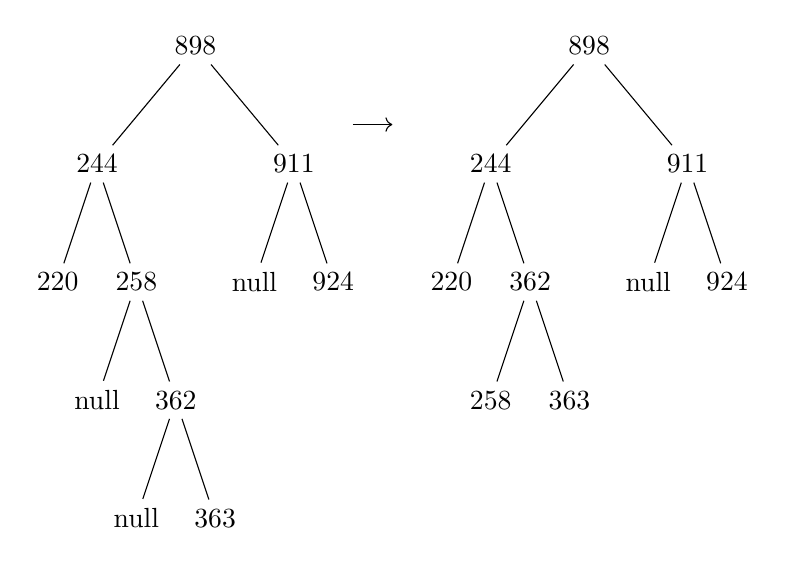
\begin{tikzpicture}
        % Primeiro arvore
        \node[shift={(0,0)}] {898}
          child[sibling distance=2.5cm] {
            node {244}
            child[sibling distance=1cm] {node {220}}
            child[sibling distance=1cm] {node {258}
              child[sibling distance=1cm] {node {null}}
              child[sibling distance=1cm] {node {362}
                child[sibling distance=1cm] {node {null}}
                child[sibling distance=1cm] {node {363}}
              }
            }
          }
          child[sibling distance=2.5cm] {
            node {911}
            child[sibling distance=1cm] {node {null}}
            child[sibling distance=1cm] {node {924}}
          };

        \draw[->] (2,-1) -- (2.5,-1);

        % Segundo arvore
        \node[shift={(5,0)}] {898}
          child[sibling distance=2.5cm] {
            node {244}
            child[sibling distance=1cm] {node {220}}
            child[sibling distance=1cm] {node {362}
              child[sibling distance=1cm] {node {258}}
              child[sibling distance=1cm] {node {363}}
            }
          }
          child[sibling distance=2.5cm] {
            node {911}
            child[sibling distance=1cm] {node {null}}
            child[sibling distance=1cm] {node {924}}
          };
    \end{tikzpicture}
  \end{center}

  \item Inserindo 360:
  \begin{center}
    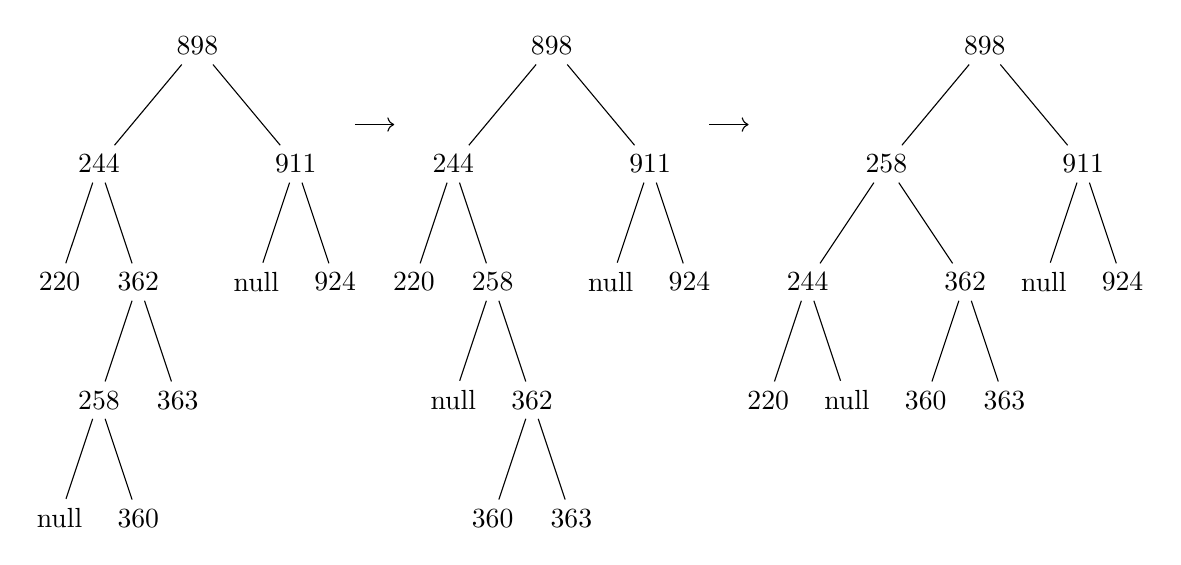
\begin{tikzpicture}
        % Primeiro arvore
        \node {898}
          child[sibling distance=2.5cm] {
            node {244}
            child[sibling distance=1cm] {node {220}}
            child[sibling distance=1cm] {node {362}
              child[sibling distance=1cm] {node {258}
                child[sibling distance=1cm] {node {null}}
                child[sibling distance=1cm] {node {360}}
              }
              child[sibling distance=1cm] {node {363}}
            }
          }
          child[sibling distance=2.5cm] {
            node {911}
            child[sibling distance=1cm] {node {null}}
            child[sibling distance=1cm] {node {924}}
          };

        \draw[->] (2,-1) -- (2.5,-1);

        % Segundo arvore
        \node[shift={(4.5,0)}] {898}
          child[sibling distance=2.5cm] {
            node {244}
            child[sibling distance=1cm] {node {220}}
            child[sibling distance=1cm] {node {258}
              child[sibling distance=1cm] {node {null}}
              child[sibling distance=1cm] {node {362}
                child[sibling distance=1cm] {node {360}}
                child[sibling distance=1cm] {node {363}}
              }
            }
          }
          child[sibling distance=2.5cm] {
            node {911}
            child[sibling distance=1cm] {node {null}}
            child[sibling distance=1cm] {node {924}}
          };
        
        \draw[->] (6.5,-1) -- (7,-1);

        % Terceiro arvore
        \node[shift={(10,0)}] {898}
          child[sibling distance=2.5cm] {
            node {258}
            child[sibling distance=2cm] {node {244}
              child[sibling distance=1cm] {node {220}}
              child[sibling distance=1cm] {node {null}}
            }
            child[sibling distance=2cm] {node {362}
              child[sibling distance=1cm] {node {360}}
              child[sibling distance=1cm] {node {363}}
            }
          }
          child[sibling distance=2.5cm] {
            node {911}
            child[sibling distance=1cm] {node {null}}
            child[sibling distance=1cm] {node {924}}
          };
    \end{tikzpicture}
  \end{center}

  \item Inserindo 350:
  \begin{center}
    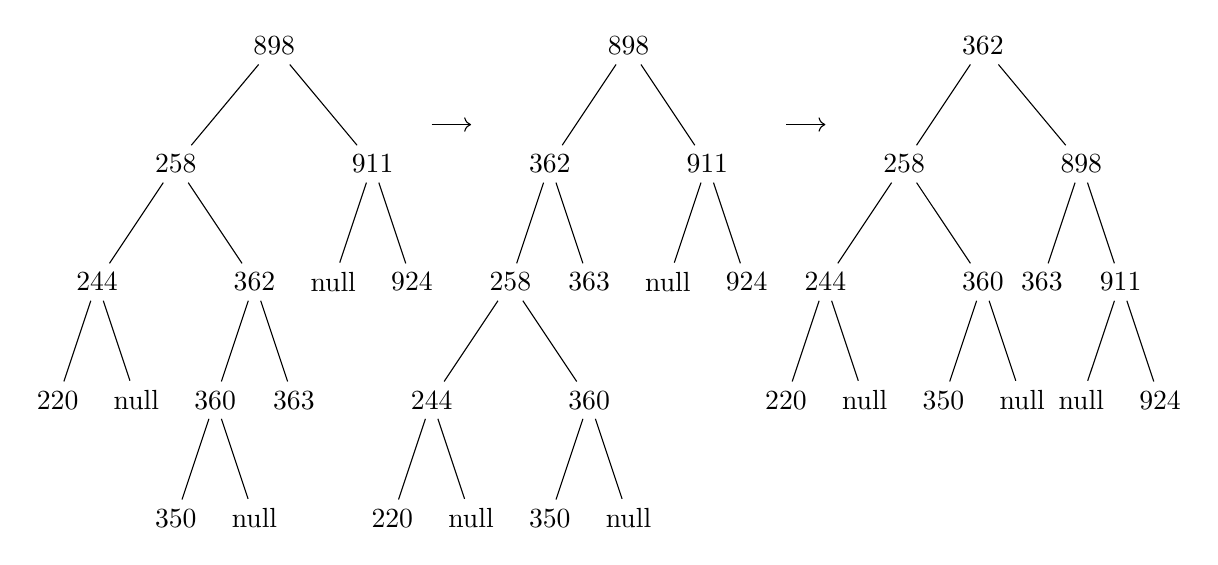
\begin{tikzpicture}
        % Primeiro arvore
        \node {898}
          child[sibling distance=2.5cm] {
            node {258}
            child[sibling distance=2cm] {node {244}
              child[sibling distance=1cm] {node {220}}
              child[sibling distance=1cm] {node {null}}
            }
            child[sibling distance=2cm] {node {362}
              child[sibling distance=1cm] {node {360}
                child[sibling distance=1cm] {node {350}}
                child[sibling distance=1cm] {node {null}}
              }
              child[sibling distance=1cm] {node {363}}
            }
          }
          child[sibling distance=2.5cm] {
            node {911}
            child[sibling distance=1cm] {node {null}}
            child[sibling distance=1cm] {node {924}}
          };

        \draw[->] (2,-1) -- (2.5,-1);

        % Segundo arvore
        \node[shift={(4.5,0)}] {898}
          child[sibling distance=2cm] {
            node {362}
            child[sibling distance=1cm] {node {258}
              child[sibling distance=2cm] {node {244}
                child[sibling distance=1cm] {node {220}}
                child[sibling distance=1cm] {node {null}}
              }
              child[sibling distance=2cm] {node {360}
                child[sibling distance=1cm] {node {350}}
                child[sibling distance=1cm] {node {null}}
              }
            }
            child[sibling distance=1cm] {node {363}}
          }
          child[sibling distance=2cm] {
            node {911}
            child[sibling distance=1cm] {node {null}}
            child[sibling distance=1cm] {node {924}}
          };
        
        \draw[->] (6.5,-1) -- (7,-1);

        % Terceiro arvore
        \node[shift={(9,0)}] {362}
          child[sibling distance=2cm] {
            node {258}
            child[sibling distance=2cm] {node {244}
              child[sibling distance=1cm] {node {220}}
              child[sibling distance=1cm] {node {null}}
            }
            child[sibling distance=2cm] {node {360}
              child[sibling distance=1cm] {node {350}}
              child[sibling distance=1cm] {node {null}}
            } 
          }
          child[sibling distance=2.5cm] {
            node {898}
            child[sibling distance=1cm] {node {363}}
            child[sibling distance=1cm] {node {911}
              child[sibling distance=1cm] {node {null}}
              child[sibling distance=1cm] {node {924}}
            }
          };
    \end{tikzpicture}
  \end{center}

\end{enumerate}

\subsubsection{c) remova o nó 362 em ambas as árvores.}

\begin{enumerate}
  \item Removendo o nó 362 da árvore binária:
  \begin{center}
    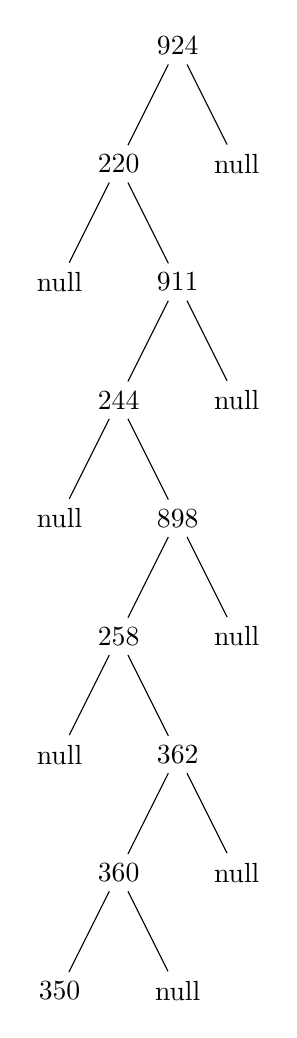
\begin{tikzpicture}
        \node {924}
            child {
              node {220}
              child {node {null}}
              child {node {911}
                child {node {244}
                  child {node {null}}
                  child {node {898}
                    child {node {258}
                      child {node {null}}
                      child {node {362}
                        child {node {360}
                          child {node {350}}
                          child {node {null}}
                        }
                        child {node {null}}
                      }
                    }
                    child {node {null}}
                  }
                }
                child {node {null}}
              }
            }
            child {
              node {null}
            };
    \end{tikzpicture}
  \end{center}

  \item Removendo o nó 362 da árvore AVL:
  \begin{center}
    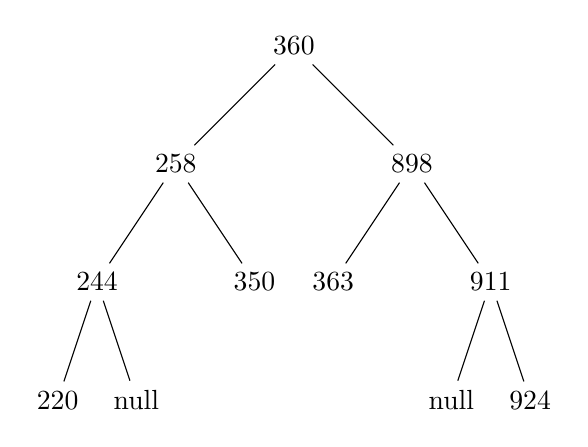
\begin{tikzpicture}
      \node[shift={(9,0)}] {360}
          child[sibling distance=3cm] {
            node {258}
            child[sibling distance=2cm] {node {244}
              child[sibling distance=1cm] {node {220}}
              child[sibling distance=1cm] {node {null}}
            }
            child[sibling distance=2cm] {node {350}} 
          }
          child[sibling distance=3cm] {
            node {898}
            child[sibling distance=2cm] {node {363}}
            child[sibling distance=2cm] {node {911}
              child[sibling distance=1cm] {node {null}}
              child[sibling distance=1cm] {node {924}}
            }
          };
    \end{tikzpicture}
  \end{center}

\end{enumerate}

\subsection {(0,2) A operação de eliminação é comutativa, ie, a eleminação de x e depois y
resulta na mesma árvore que a eliminação de y e depois x? Mostre um contra-
exemplo.}

\subsubsection{Solução:}

Fonte: https://www.cs.cornell.edu/courses/cs409/2000SP/Homework/hw03Solution.htm
\\
\\
Delete não é comutativo. O exemplo abaixo usa a regra de que a exclusão de um nó com dois filhos é feita excluindo seu sucessor.

\begin{enumerate}
  \item Removendo o nó 50 depois a nó 30:
  \begin{center}
    \begin{tikzpicture}
        % Primeiro arvore
        \node {50}
          child[sibling distance=2cm] {
            node {30}
          }
          child[sibling distance=2cm] {
            node {70}
            child[sibling distance=1cm] {node {60}}
            child[sibling distance=1cm] {node {null}}
          };

        \draw[->] (1.5,-1) -- (2,-1);

        % Segundo arvore
        \node[shift={(4,0)}] {60}
          child[sibling distance=2cm] {
            node {30}
          }
          child[sibling distance=2cm] {
            node {70}
          };
        
        \draw[->] (6,-1) -- (6.5,-1);

        % Terceiro arvore
        \node[shift={(8,0)}] {60}
          child[sibling distance=2cm] {
            node {null}
          }
          child[sibling distance=2.5cm] {
            node {70}
          };
    \end{tikzpicture}
  \end{center}

  \item Removendo o nó 30 depois a nó 50:
  \begin{center}
    \begin{tikzpicture}
        % Primeiro arvore
        \node {50}
          child[sibling distance=2cm] {
            node {30}
          }
          child[sibling distance=2cm] {
            node {70}
            child[sibling distance=1cm] {node {60}}
            child[sibling distance=1cm] {node {null}}
          };

        \draw[->] (1.5,-1) -- (2,-1);

        % Segundo arvore
        \node[shift={(4,0)}] {50}
          child[sibling distance=2cm] {
            node {null}
          }
          child[sibling distance=2cm] {
            node {70}
            child[sibling distance=1cm] {node {60}}
            child[sibling distance=1cm] {node {null}}
          };
        
        \draw[->] (6,-1) -- (6.5,-1);

        % Terceiro arvore
        \node[shift={(8,0)}] {70}
          child[sibling distance=2cm] {
            node {60}
          }
          child[sibling distance=2.5cm] {
            node {null}
          };
    \end{tikzpicture}
  \end{center}

\end{enumerate}

\subsection {(0,4) Escreva o código de remoção em árvore AVL. Explique quais são as principais
diferenças comparadas ao algoritmo de remoção em árvore binária.}

\subsubsection{Solução:}

Fonte: ChatGPT
\\
\\
A remoção em uma árvore AVL segue o mesmo princípio de remoção de uma árvore binária de busca (BST - Binary Search Tree), 
mas com o adicional de reequilibrar a árvore após a remoção, para manter a propriedade de balanceamento da árvore AVL, 
onde a diferença de altura entre as subárvores esquerda e direita de qualquer nó não pode ser maior que 1.

\begin{lstlisting}
# FONTE: ChatGPT
class Node:
  def __init__(self, key):
    self.key = key
    self.left = None
    self.right = None
    self.height = 1

class AVLTree:
    
  # Fun\c{c}ão para calcular a altura de um nó
  def get_height(self, node):
    if not node:
      return 0
    return node.height

  # Fun\c{c}ão para calcular o fator de balanceamento
  def get_balance(self, node):
    if not node:
      return 0
    return self.get_height(node.left) - self.get_height(node.right)

  # Rota\c{c}ão à direita
  def rotate_right(self, y):
    x = y.left
    T2 = x.right

    # Realiza a rota\c{c}ão
    x.right = y
    y.left = T2

    # Atualiza as alturas
    y.height = 1 + max(self.get_height(y.left), self.get_height(y.right))
    x.height = 1 + max(self.get_height(x.left), self.get_height(x.right))

    # Retorna a nova raiz
    return x

  # Rota\c{c}ão à esquerda
  def rotate_left(self, x):
    y = x.right
    T2 = y.left

    # Realiza a rota\c{c}ão
    y.left = x
    x.right = T2

    # Atualiza as alturas
    x.height = 1 + max(self.get_height(x.left), self.get_height(x.right))
    y.height = 1 + max(self.get_height(y.left), self.get_height(y.right))

    # Retorna a nova raiz
    return y

  # Fun\c{c}ão para inserir um nó (usada para criar a árvore antes da remo\c{c}ão)
  def insert(self, root, key):
    if not root:
      return Node(key)
    elif key < root.key:
      root.left = self.insert(root.left, key)
    else:
      root.right = self.insert(root.right, key)

    # Atualiza a altura do nó pai
    root.height = 1 + max(self.get_height(root.left), self.get_height(root.right))

    # Verifica o balanceamento
    balance = self.get_balance(root)

    # Caso LL
    if balance > 1 and key < root.left.key:
      return self.rotate_right(root)

    # Caso RR
    if balance < -1 and key > root.right.key:
      return self.rotate_left(root)

    # Caso LR
    if balance > 1 and key > root.left.key:
      root.left = self.rotate_left(root.left)
      return self.rotate_right(root)

    # Caso RL
    if balance < -1 and key < root.right.key:
      root.right = self.rotate_right(root.right)
      return self.rotate_left(root)

    return root

  # Fun\c{c}ão para encontrar o nó com valor mínimo (usada durante a remo\c{c}ão)
  def find_min_value_node(self, node):
    current = node
    while current.left is not None:
      current = current.left
    return current

  # Fun\c{c}ão para remover um nó em uma árvore AVL
  def remove(self, root, key):
    # Passo 1: Realiza a remo\c{c}ão padrão da árvore binária de busca
    if not root:
      return root
    elif key < root.key:
      root.left = self.remove(root.left, key)
    elif key > root.key:
      root.right = self.remove(root.right, key)
    else:
      # Nó encontrado, realiza a remo\c{c}ão
      if root.left is None:
          temp = root.right
          root = None
          return temp
      elif root.right is None:
          temp = root.left
          root = None
          return temp

      # Nó com dois filhos: pegar o sucessor in-order
      temp = self.find_min_value_node(root.right)
      root.key = temp.key
      root.right = self.remove(root.right, temp.key)

    # Se a árvore tiver apenas um nó, retorna
    if root is None:
      return root

    # Passo 2: Atualiza a altura do nó atual
    root.height = 1 + max(self.get_height(root.left), self.get_height(root.right))

    # Passo 3: Calcula o fator de balanceamento
    balance = self.get_balance(root)

    # Passo 4: Verifica se o nó está desbalanceado e realiza rota\c{c}ões apropriadas

    # Caso LL
    if balance > 1 and self.get_balance(root.left) >= 0:
      return self.rotate_right(root)

    # Caso LR
    if balance > 1 and self.get_balance(root.left) < 0:
      root.left = self.rotate_left(root.left)
      return self.rotate_right(root)

    # Caso RR
    if balance < -1 and self.get_balance(root.right) <= 0:
      return self.rotate_left(root)

    # Caso RL
    if balance < -1 and self.get_balance(root.right) > 0:
      root.right = self.rotate_right(root.right)
      return self.rotate_left(root)

    return root

\end{lstlisting}

Principais Diferenças:
  \begin{enumerate}[label=\alph*)]
    \item Balanceamento: A árvore AVL mantém um fator de balanceamento (dife-rença de alturas entre as subárvores esquerda e direita) de nó máximo 1, realizando rotações após a remoção para garantir essa propriedade. A árvore binária comum não possui essa garantia.
    \item Rotações: Na árvore AVL, podem ser necessárias rotações para corrigir o balanceamento após a remoção, o que não ocorre em árvores binárias de busca simples.
    \item Eficiência: Devido ao balanceamento, a árvore AVL mantém sua altura controlada em O(log n), enquanto a árvore binária de busca pode crescer desbalanceada, levando a uma altura O(n) no pior caso.
  \end{enumerate}
\end{document}